\subsection{Use case diagram}
	A global picture of the system interaction with actors is provided here by means of use case diagrams. Following, an analysis of the most interesting use case situations derived from scenarios is presented.

	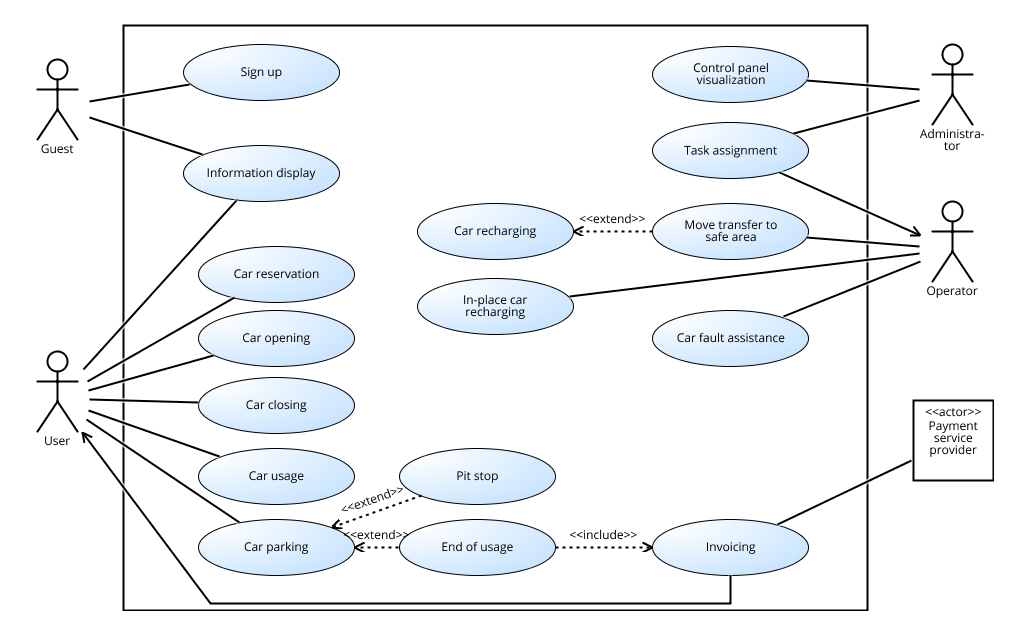
\includegraphics[width=\textwidth]{img/use_case.png}

	\subsubsection{Use case 1: Reserve a car}
		\begin{description}
			\item[Name] Reserve a car
			\item[Actors] \hfill
				\begin{description}
					\item[User] The user who wants to reserve a car
				\end{description}
			\item[Entry condition] The user decides to reserve a car to take in the next hour.
			\item[Flow of events] \hfill
				\begin{enumerate}
					\item The user logs in into the mobile app and goes to the reservation section. \item The system automatically retrieves and displays the location of the user, but they can specify a different location if needed.
					\item The system displays the position of the available cars close to the selected location.
					\item The user selects a car and confirm the reservation.
				\end{enumerate}
			\item[Exit condition] The system reserves the car for the user.
			\item[Exceptions] \hfill
				\begin{itemize}
					\item \textbf{The system is not able to locate the user automatically.} The user is required to insert a position manually.
					\item \textbf{The system is not able to find a position inserted manually.} The user is informed and the operation is aborted.
					\item \textbf{There are no available cars.} The user is informed and the operation is aborted.
					\item \textbf{The user cancels the operation before confirming.} The reservation process is not completed and the car remains available to other users.
				\end{itemize}
			\item[Special Requirements] None.

%Name of Use Case
%Actors
%Description of Actors involved in use case)
%Entry condition
%“This use case starts when...”
%Flow of Events
%Free form, informal natural language
%Exit condition
%“This use cases terminates when...”
%Exceptions
%Describe what happens if things go wrong
%Special Requirements
%Nonfunctional Requirements, Constraints)
		\end{description}